\chapter{Results}

The aim of the methods described in this thesis is to provide tools to query the disequilibrium of sequence evolution. Described in this chapter is the characterisation of the developed methods. I present two new statistics for measuring the magnitude of disequilibrium. I evaluate these statistics on simulated data. I present the application of the test of existence, and test of consistency to simulated data. I complement this with the results of the methods applied to empirical data where I expect disequilibrium to exist.

\section{Methods of Quantifying Disequilibrium}






\section{Is the Human Genome at Equilibrium?}

\begin{figure}[h]
\centering
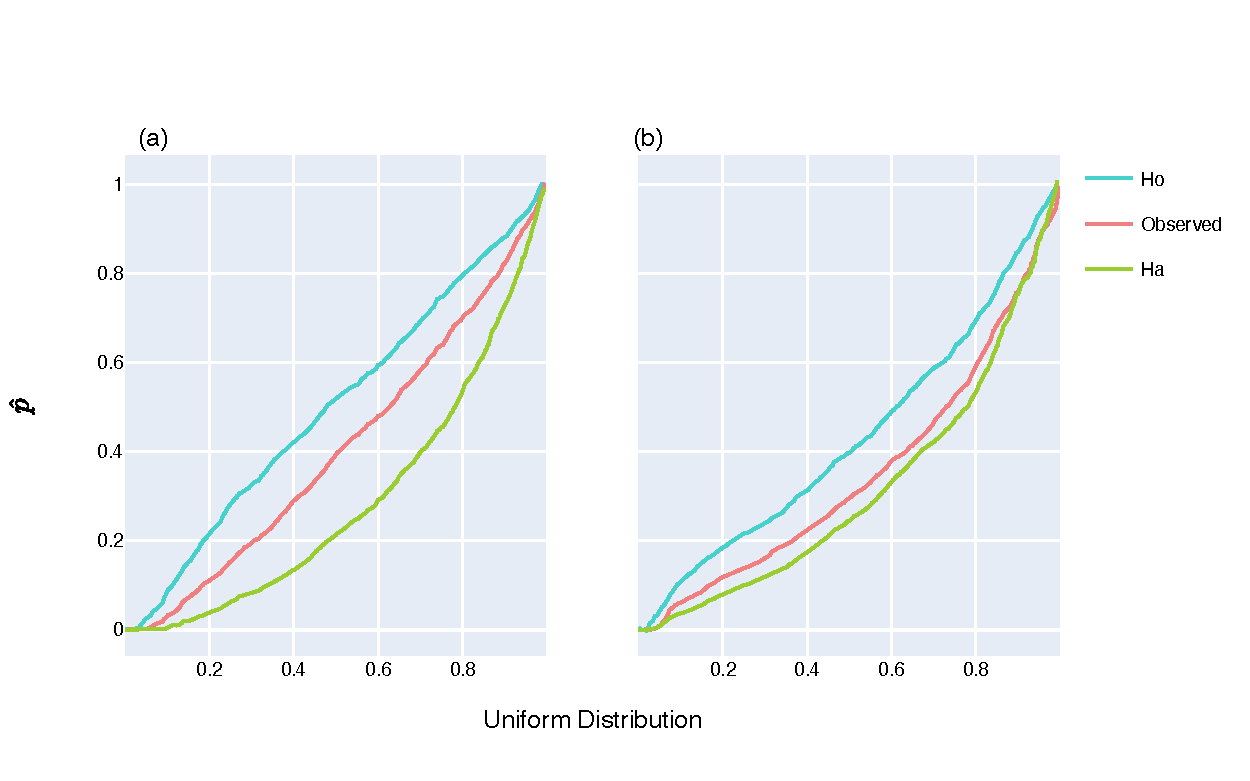
\includegraphics[width=	\textwidth]{figures/plots/primate/LRT-QQ.pdf}
\caption[Humans exhibit a higher proportion of mutation disequilibrium in CDS compared to introns]{\textbf{Humans exhibit a higher proportion of mutation disequilibrium in CDS compared to introns.} The Quantile-Quantile plots compare the distribution of $\hat p-$values to the expected uniform distribution. \textbf{(a)} 1,406 alignments of introns from human, chimpanzee and gorilla, \textbf{(b)}, 1,182 CDS alignments from human, chimpanzee and gorilla. For all model fitting human was the foreground edge. }
\label{fig:primate_lrt_qq}
\end{figure}




Rates of evolution in introns and exons. If the null was true, and the branch length was the same between introns and exons, then the distribution of the difference would be centered on zero. Try a T-test of the null that the mean is zero, against the prior alternate that the exons are evolving slower, and so the mean is greater than zero. The assumption of the T-test is that the distribution is normal, which is hard to say in this case. The T-test is pretty robust, but I can test for whether it is normally distributed also. 






 
\section{The PAR-half of \textit{Fxy} is further from equilibrium than the non-PAR half in \textit{M. musculus}}